

 % Copyright 2004 by Till Tantau <tantau@users.sourceforge.net>.
%
% In principle, this file can be redistributed and/or modified under
% the terms of the GNU Public License, version 2.
%
% However, this file is supposed to be a template to be modified
% for your own needs. For this reason, if you use this file as a
% template and not specifically distribute it as part of a another
% package/program, I grant the extra permission to freely copy and
% modify this file as you see fit and even to delete this copyright
% notice. 

\documentclass{beamer}

% There are many different themes available for Beamer. A comprehensive
% list with examples is given here:
% http://deic.uab.es/~iblanes/beamer_gallery/index_by_theme.html
% You can uncomment the themes below if you would like to use a different
% one:
%\usetheme{AnnArbor}
%\usetheme{Antibes}
%\usetheme{Bergen}
%\usetheme{Berkeley}
%\usetheme{Berlin}
%\usetheme{Boadilla}
%\usetheme{boxes}
%\usetheme{CambridgeUS}
%\usetheme{Copenhagen}
%\usetheme{Darmstadt}
%\usetheme{default}
%\usetheme{Frankfurt}
%\usetheme{Goettingen}
%\usetheme{Hannover}
%\usetheme{Ilmenau}
%\usetheme{JuanLesPins}
%\usetheme{Luebeck}
\usetheme{Madrid}
%\usetheme{Malmoe}
%\usetheme{Marburg}
%\usetheme{Montpellier}
%\usetheme{PaloAlto}
%\usetheme{Pittsburgh}
%\usetheme{Rochester}
%\usetheme{Singapore}
%\usetheme{Szeged}
%\usetheme{Warsaw}


% Customize Warsaw color 
\setbeamercolor*{palette primary}{use=structure,fg=white,bg=red!50!black}
\setbeamercolor*{palette secondary}{use=structure,fg=white,bg=red!60!black}
\setbeamercolor*{palette tertiary}{use=structure,fg=white,bg=red!70!black}

% Customize Warsaw block title and background colors
\setbeamercolor{block title}{bg=red!50!black,fg=white}


\usepackage{siunitx}
\sisetup{unitsep=\cdot}

\usepackage{epstopdf}
\epstopdfsetup{suffix={}}

\title[BEMOSS (Proposal)]{Building Energy Management Internet of Things}

% % A subtitle is optional and this may be deleted
% \subtitle{Product Proposal}

\author[R.~Bachman, R.~O'Malley, J.~Ingram]{Reece~Bachman \and Robert~O'Malley \and Jordan~Ingram \and
Advisor: Dr. Suruz Miah}
% - Give the names in the same order as the appear in the paper.
% - Use the \inst{?} command only if the authors have different
%   affiliation.

%\institute[Bradley University] % (optional, but mostly needed)
%{
%  Department of Electrical and Computer Engineering\\
%  Bradley University\\
%  1501 W. Bradley Avenue\\
%  Peoria, IL, 61625, USA
%}
% - Use the \inst command only if there are several affiliations.
% - Keep it simple, no one is interested in your street address.

\date[November~5,~2018]{Monday, November~5,~2018}
% - Either use conference name or its abbreviation.
% - Not really informative to the audience, more for people (including
%   yourself) who are reading the slides online

\logo{\hfill\href{http://www.bradley.edu}{
\includegraphics[width=0.75cm]{figs/logoBU1-Print}}}  % place logo in every page 


\subject{Building Energy Management}
% This is only inserted into the PDF information catalog. Can be left
% out. 

% If you have a file called "university-logo-filename.xxx", where xxx
% is a graphic format that can be processed by latex or pdflatex,
% resp., then you can add a logo as follows:

% \pgfdeclareimage[height=0.5cm]{university-logo}{university-logo-filename}
% \logo{\pgfuseimage{university-logo}}

% Delete this, if you do not want the table of contents to pop up at
% the beginning of each subsection:
\AtBeginSubsection[]
{
  \begin{frame}<beamer>{Outline}
    \tableofcontents[currentsection,currentsubsection]
  \end{frame}
}

% Let's get started
\begin{document}

\begin{frame}
  \titlepage
\end{frame}

\begin{frame}{Outline}
  \tableofcontents
  % You might wish to add the option [pausesections]
\end{frame}

% Section and subsections will appear in the presentation overview
% and table of contents.
\section{Introduction}

\begin{frame}{Introduction}{}
  % applications of mobile robot navigation and problem description
  \begin{itemize}
        \item Building Energy Management Open Source Software (BEMOSS) is an open source Internet of Thing (IoT) software developed under the Department of Energy 
        \item We are tasked with creating a new device that can be controlled through this software over the internet 
        \item We are creating an interface to control a DC motor through BEMOSS
        \begin{itemize}
            \item Control curtains to regulate interior temperatures
            \item Close/ open barriers
            \end{itemize}
        \item We will also create a machine learning algorithm that can be supported within BEMOSS to reduce power consumption
        \end{itemize}
\end{frame}

%----------------------------------

\section{Background Study}

\subsection{Literature}

\begin{frame}{Background Study}{Literature}
    \begin{itemize}
        \item The previous literature that has been released on BEMOSS has been describing what it can do instead of how to do it
        \item Currently BEMOSS is being used by Virginia Tech and McNeese University to monitor a microgrid
    \end{itemize}
\end{frame}

%----------------------------------

\subsection{Prior Work}

\begin{frame}{Background Study}{Prior Work}
    \begin{itemize}
      \item The BEMOSS team has thus far successfully incorporated control of the following devices into BEMOSS: 
    \end{itemize}
      \begin{figure}
  %    \boxed{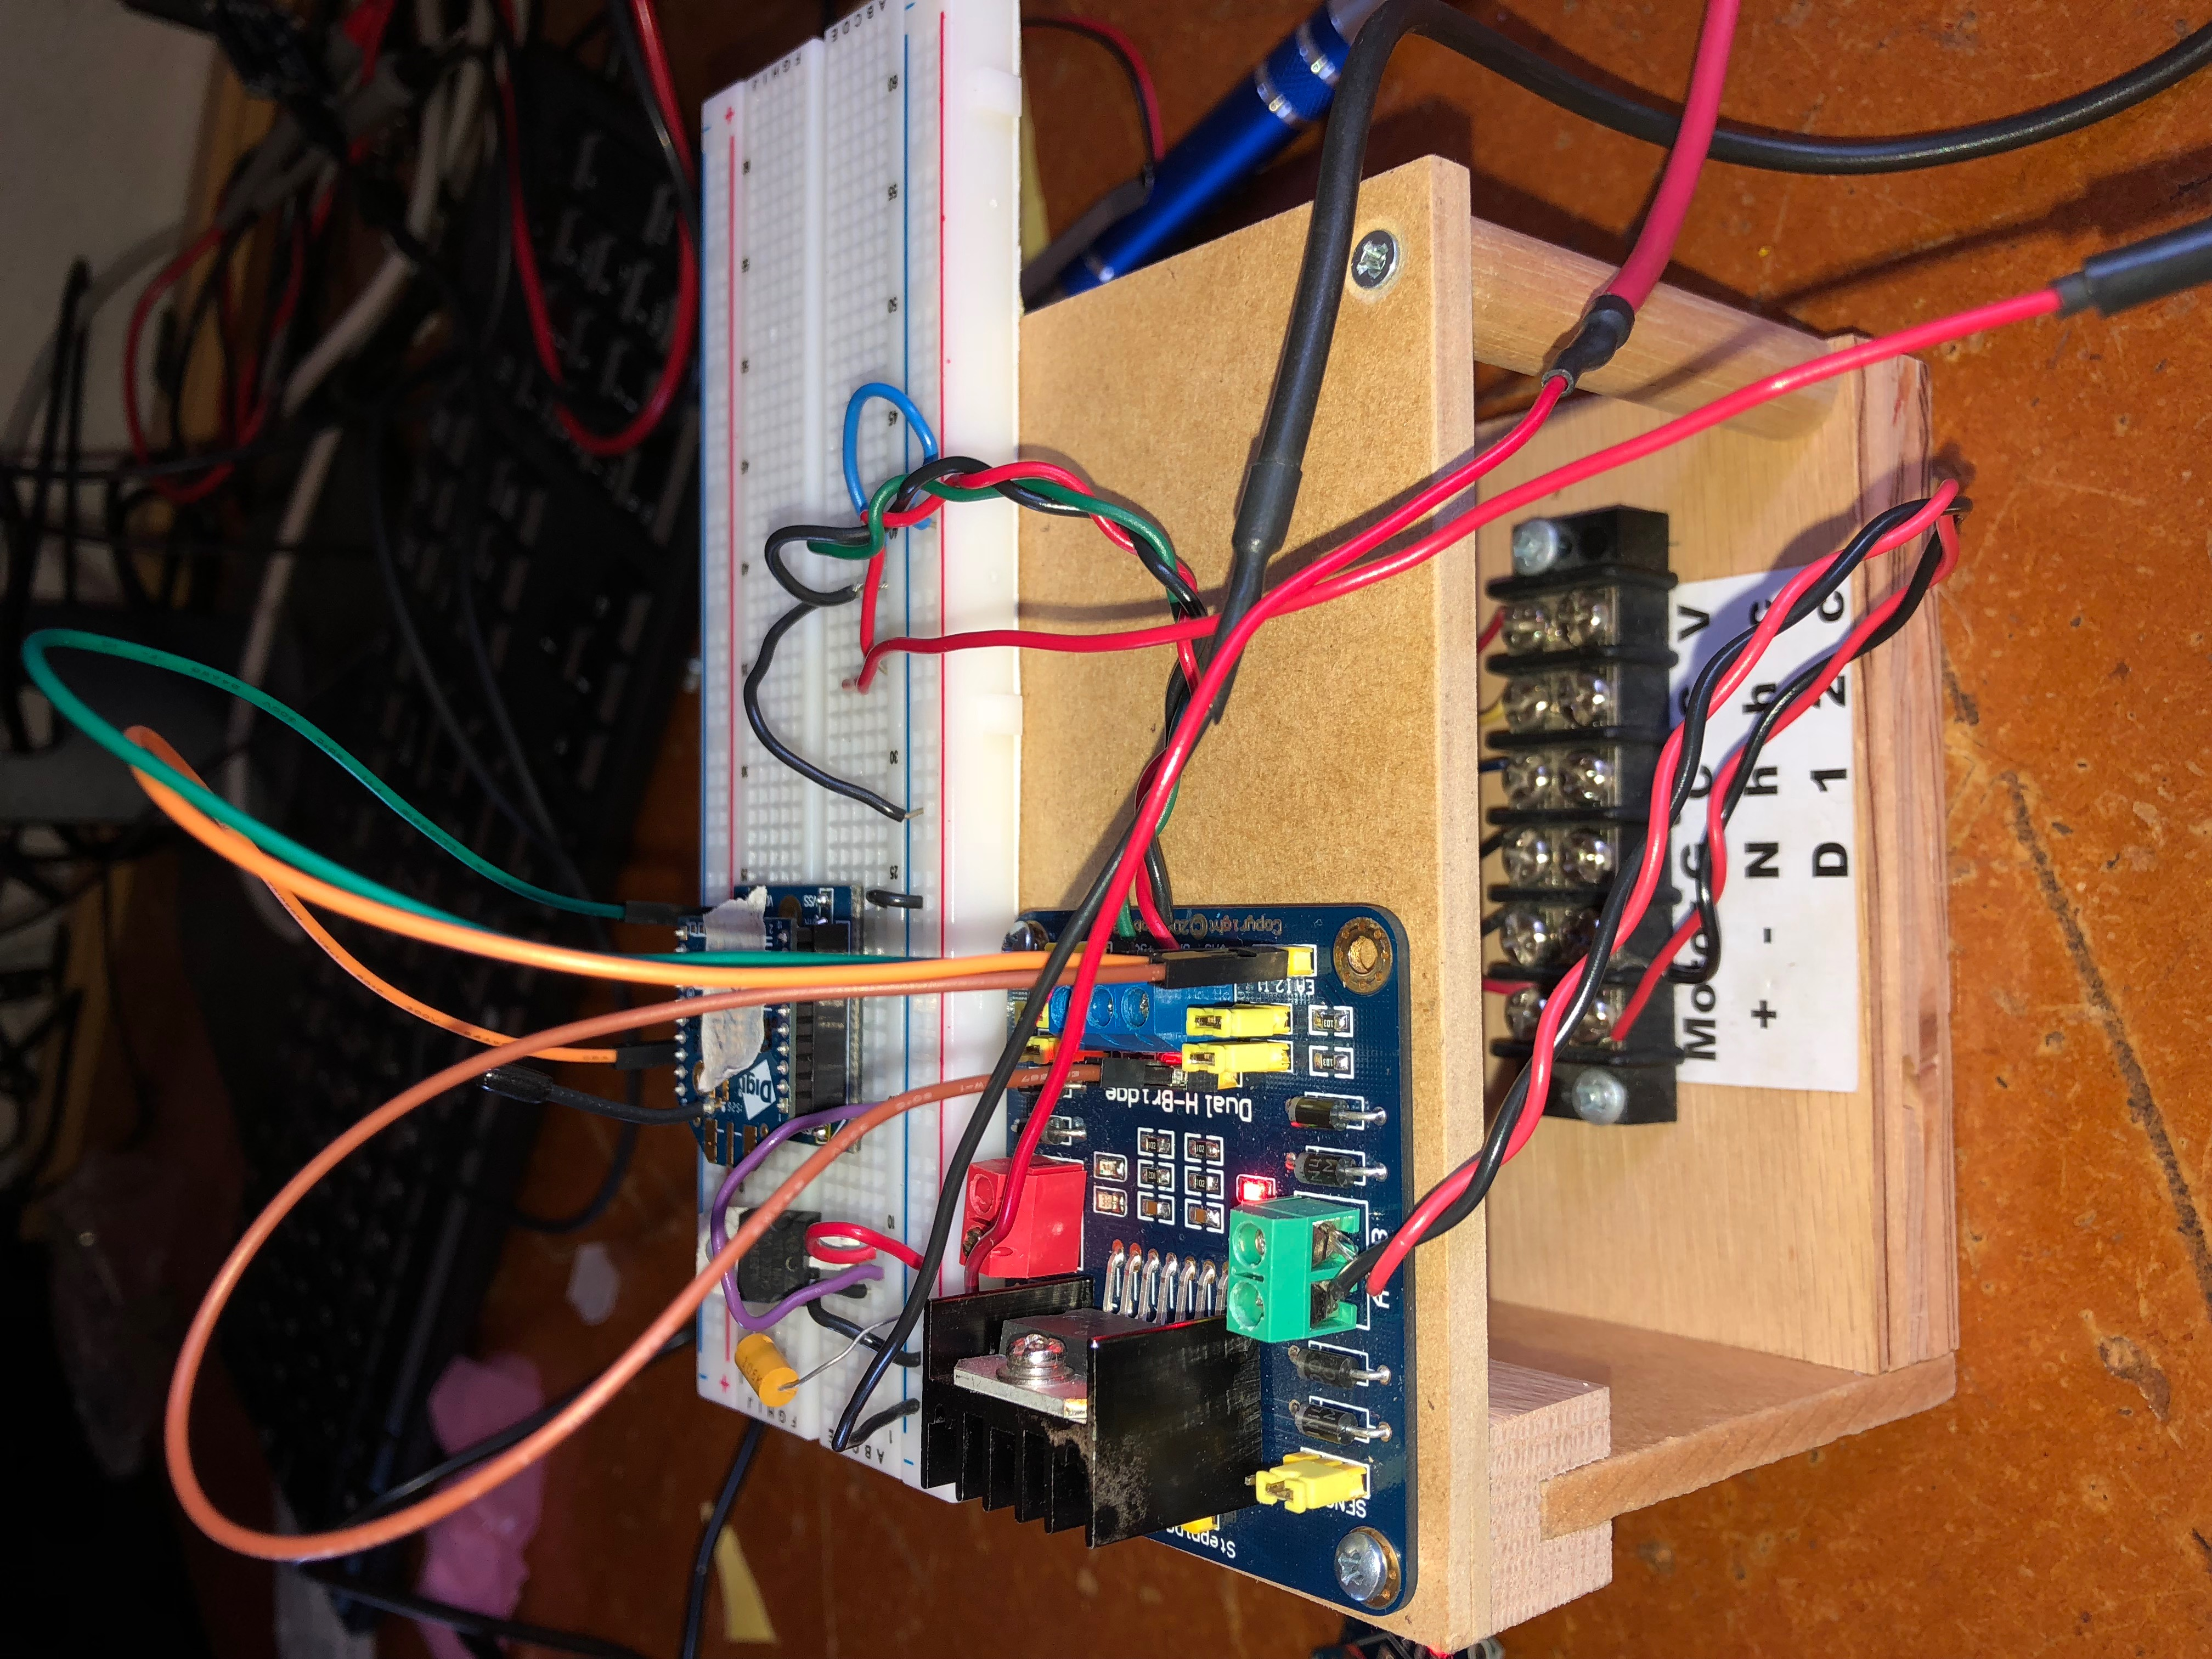
\includegraphics[width=0.5\textwidth]{labNotebookSeniorProject1-Latex2018/figs/img/Circuit10_29}}
 % \caption{Remote Motor circuit}
  \label{fig:Remote Motor Circuit}
  \boxed{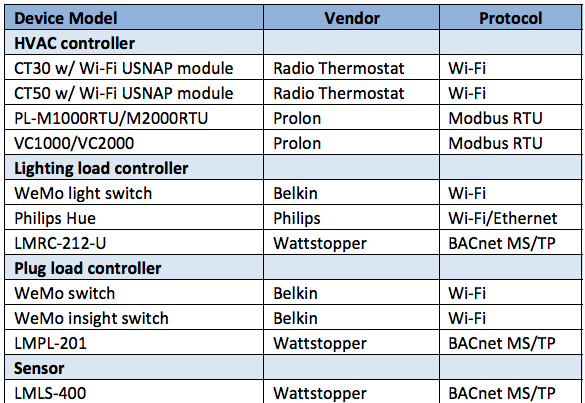
\includegraphics[width=0.5\textwidth]{figs/img/BemossSuportedDevices.png}}
        \end{figure}
    

\end{frame}
%----------------------------------

\subsection{Challenges}
 %http://www.bemoss.org/supported_devices_hardware/
\begin{frame}{Background Study}{Challenges}
    \begin{itemize}
        \item Create a new BEMOSS supported device
        \item Implement BEMOSS on a new device, such as a raspberry pi
        \item Develop and implement an algorithm for BEMOSS to use to efficiently utilize power consumption in a HVAC system 
    \end{itemize}
  
\end{frame}

%----------------------------------

\section{Subsystem Level Functional Requirements}

% put a slide with three dimensional system architecture drawing using ipe
% another slide with explanation

% put a slide with system block diagram

\subsection{Block Diagram}

\begin{frame}{Subsystem Level Functional Requirements}{Block Diagram}
\begin{figure}
      \label{fig:Motor Block Diagram}
      \boxed{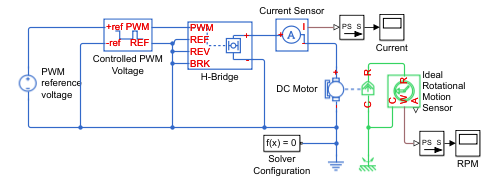
\includegraphics[width=0.95\textwidth]{figs/img/motorModelWithHBridge.png}}
\end{figure}

\end{frame}

%\subsection{Block Diagram}


%----------------------------------

\subsection{Specifications}

\begin{frame}{Subsystem Level Functional Requirements}{Specifications}
Motor Requirements
\begin{itemize}
    \item The simulation must be modeled based on the real system in the lab
    \item The model must be run by a PWM signal and H-bridge to allow for feedback control later
    \item The model must produce a power calculation to be used later for the machine learning algorithm
\end{itemize}
\end{frame}

%----------------------------------

\section{Engineering Efforts}

\subsection{Simulation}

\begin{frame}{Engineering Efforts}{Simulation}
  \begin{figure}
      \label{fig:Motor Simulation Results}
      \boxed{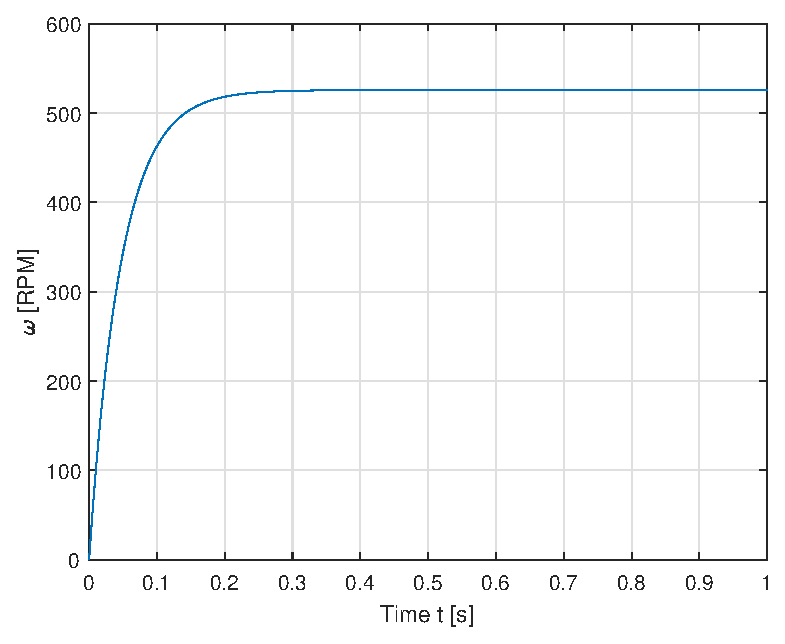
\includegraphics[width=0.65\textwidth]{figs/ipe/motorRPM.eps}}
      \caption{Motor Simulation Results}
\end{figure}
\end{frame}


%----------------------------------
\section{Subsystem Level Functional Requirements}
\subsection{Block Diagram}
\begin{frame}{Subsystem Level Functional Requirements}{Block Diagram}
\begin{figure}
      \label{fig:House HVAC Model}
      \boxed{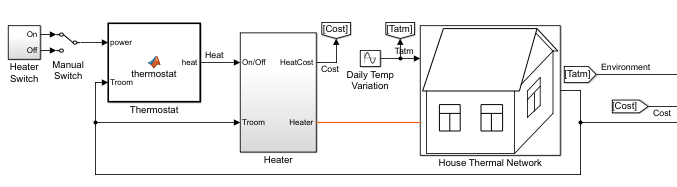
\includegraphics[width=0.95\textwidth]{figs/img/houseModel.PNG}}
\end{figure}
\end{frame}

%----------------------------------
\subsection{Specifications}
\begin{frame}{Subsystem Level Functional Requirements}{Specifications}
House Requirements
\begin{itemize}
    \item The model must give a realistic thermal behavior of a room
    \item Modeled after work done by a previous work, the system is modeled after the system of equations:
\end{itemize}
\begin{multline*}
    \label{eq:HVAC-Modeling}
    \frac{\mathrm{d}\mathbf{T}^e}{\mathrm{dt}} = 
    \begin{bmatrix}
    \dot{T}_1^e\\
    \dot{T}_2^e    
    \end{bmatrix}
    = 
    \begin{bmatrix}
    -\frac{u_{cc}A_{cc}}{M_{cc}C_v} & \frac{Q_w\rho_w C_{\rho_w}}{M_{cc}C_v}\\
    0 &  -\frac{Q_w\rho_wC_{pw}+U_tA_t}{V_t\rho_wC_{pw}}
    \end{bmatrix}
    \begin{bmatrix}
    T_1^e\\
    T_2^e
    \end{bmatrix}
    +\\
    \begin{bmatrix}
    \frac{U_{cc}A_{cc}}{M_{cc}C_v}T_{amb} - \frac{Q_w\rho_wC_{pw}}{M_{cc}C_v}T_{wo} \\
    \frac{U_tA_t}{V_t\rho_wC_{pw}}T_{amb} + \frac{Q_w\rho_wC_{pw}}{V_t\rho_wC_{pw}}T_{wo}
    \end{bmatrix}
    +
    \begin{bmatrix}
    0 \\
    \frac{15000}{V_t\rho_wC_{pw}}
    \end{bmatrix}
    \chi
    +
    \begin{bmatrix}
    (\frac{\rho_aC_{pa}}{M_{cc}C_v}Q_{a1}-\frac{U_{cc}A_{cc}}{M_{cc}C_v})\\
    0
    \end{bmatrix}    
\end{multline*}
\end{frame}
%----------------------------------
\section{Engineering Efforts}
\subsection{Simulation}
\begin{frame}{Engineering Efforts}{Simulation}
  \begin{figure}
      \label{fig:House Simulation Results}
      \boxed{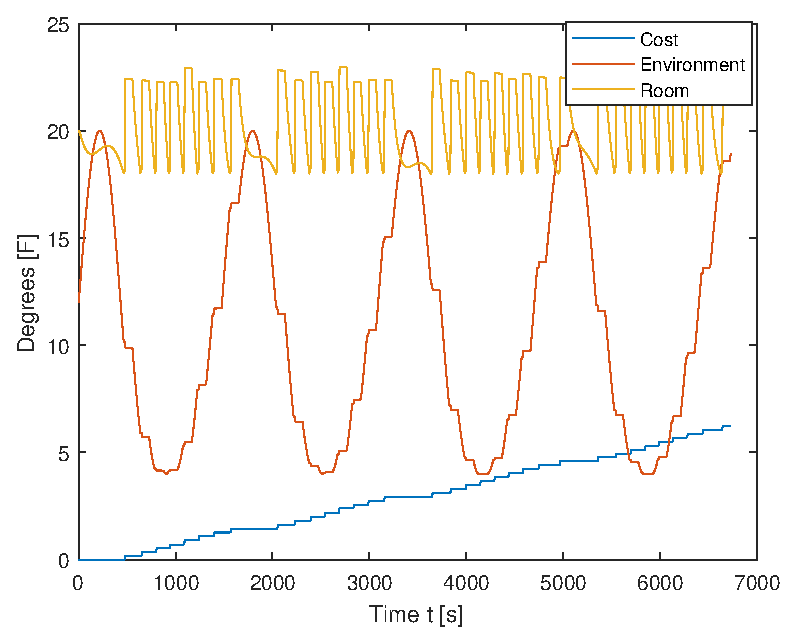
\includegraphics[width=0.65\textwidth]{figs/ipe/houseModel.eps}}
      \caption{House Simulation Results using on/off control}
\end{figure}
\end{frame}
%----------------------------------
\subsection{Design}

\begin{frame}{Engineering Efforts}{Design}
  \begin{figure}
    \centering
    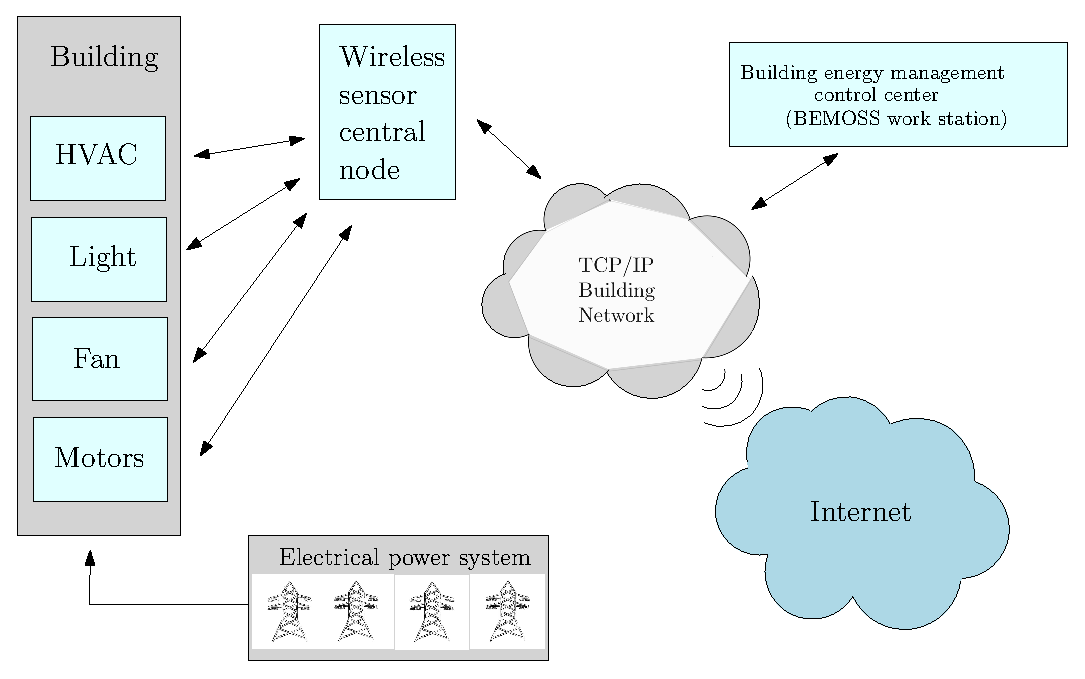
\includegraphics[scale=.6]{figs/ipe/HighLevelBemoss.eps}
    \caption{BEMOSS Network}
    \label{fig:BEMOSS Network}
\end{figure}
\end{frame}

\begin{frame}{Engineering Efforts}{Design}
  Hardware video demonstration 
\end{frame}


\begin{frame}{Engineering Efforts}{Design}
  \begin{figure}
    \centering
    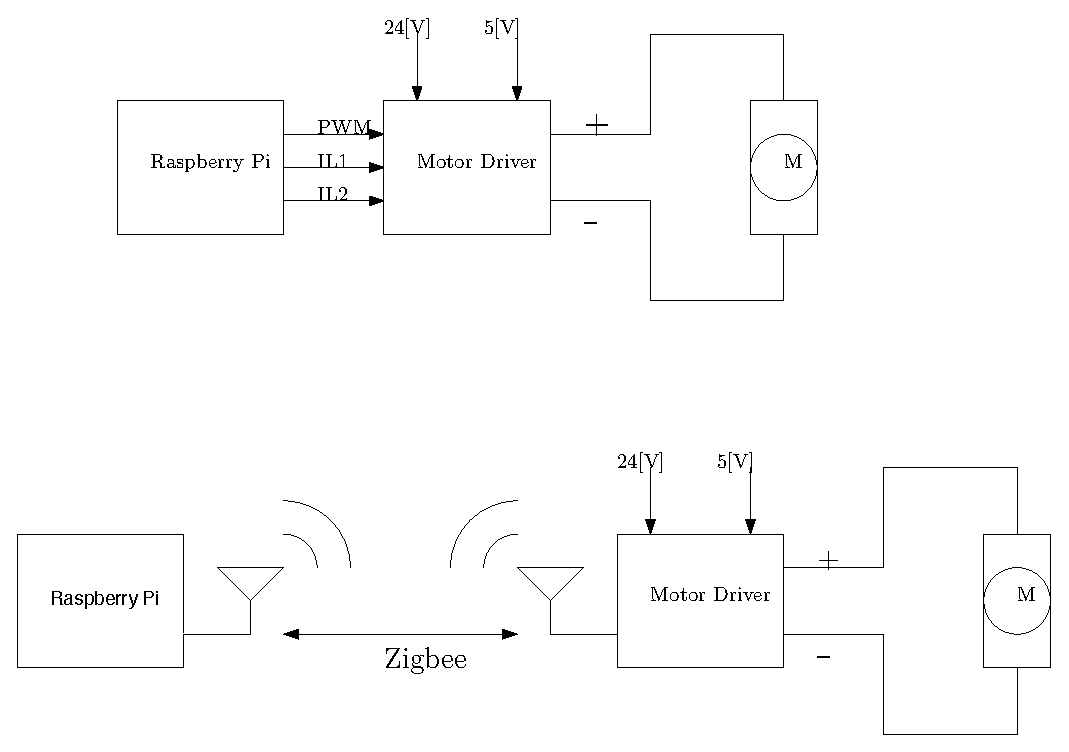
\includegraphics[scale=.5]{figs/ipe/RpiMDInterface.eps}
    \caption{Raspberry Pi Motor Driver Interface}
    \label{fig:RpiMDInterface}
\end{figure}
\end{frame}

%----------------------------------

\subsection{Experimental Activities}


   % 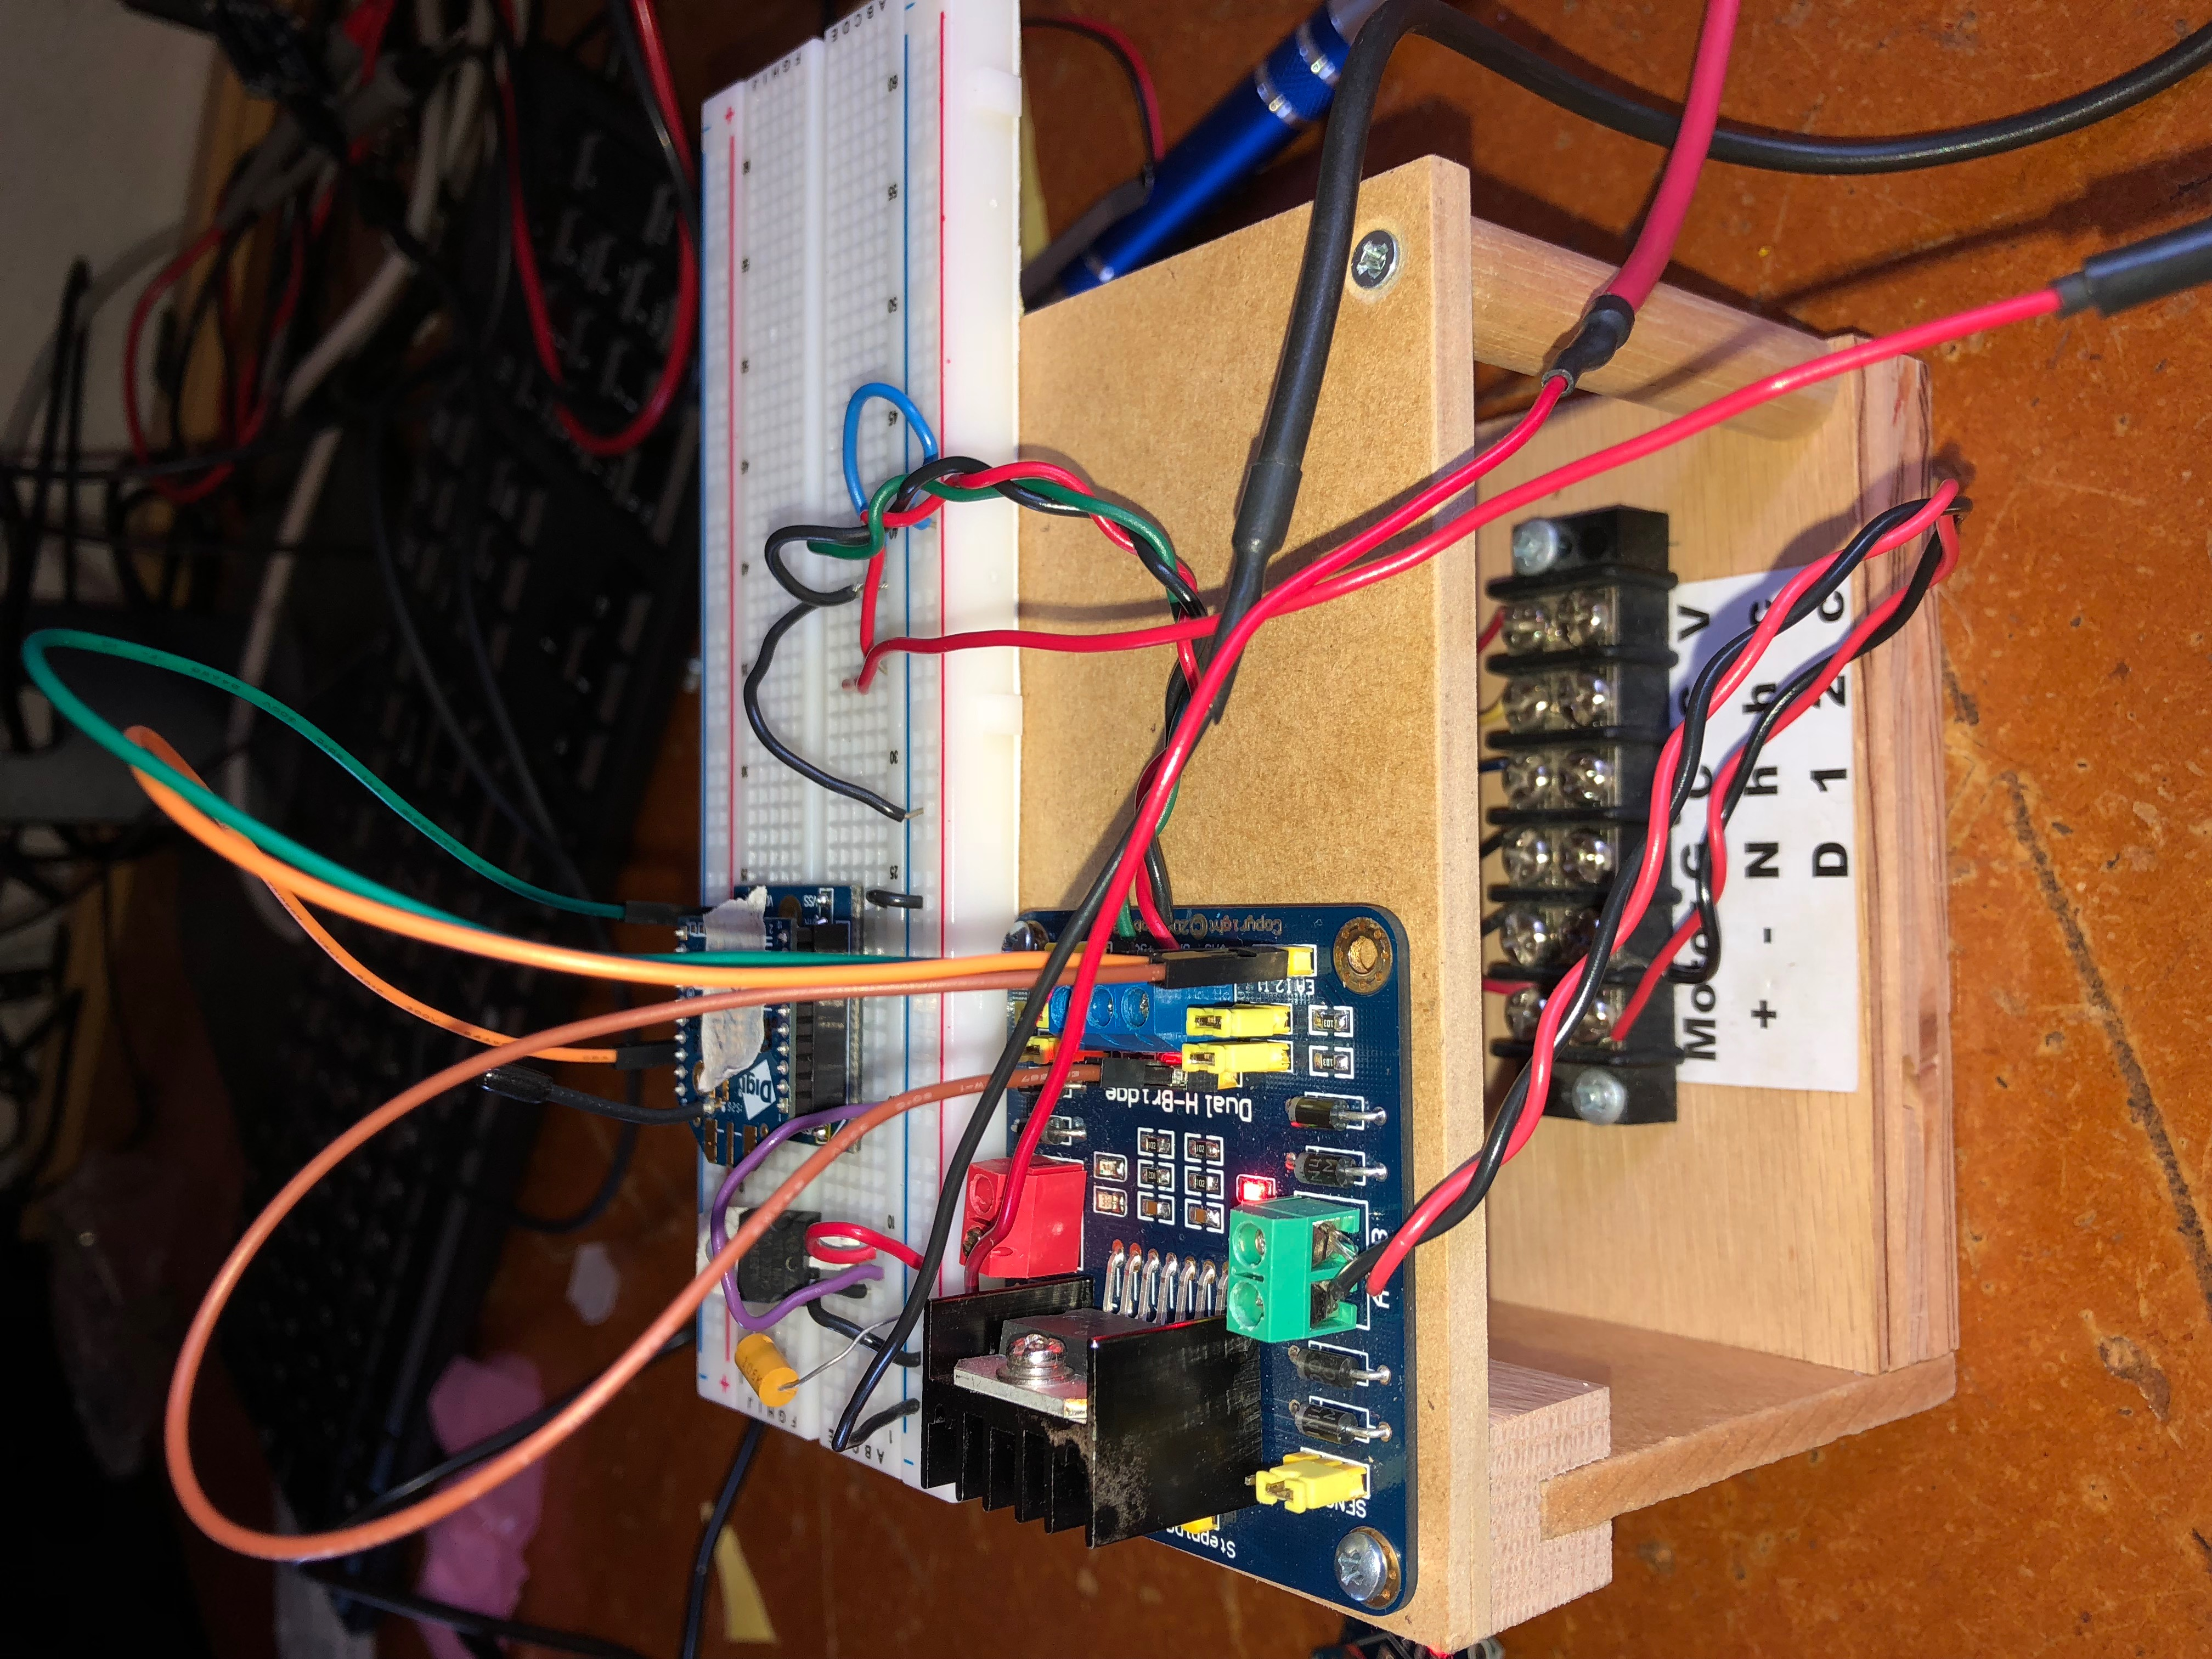
\includegraphics[scale=.04, angle =270]{figs/Circuit.jpg}

\begin{frame}{Engineering Efforts}{Experimental Activities}
     \begin{figure}
     \centering
     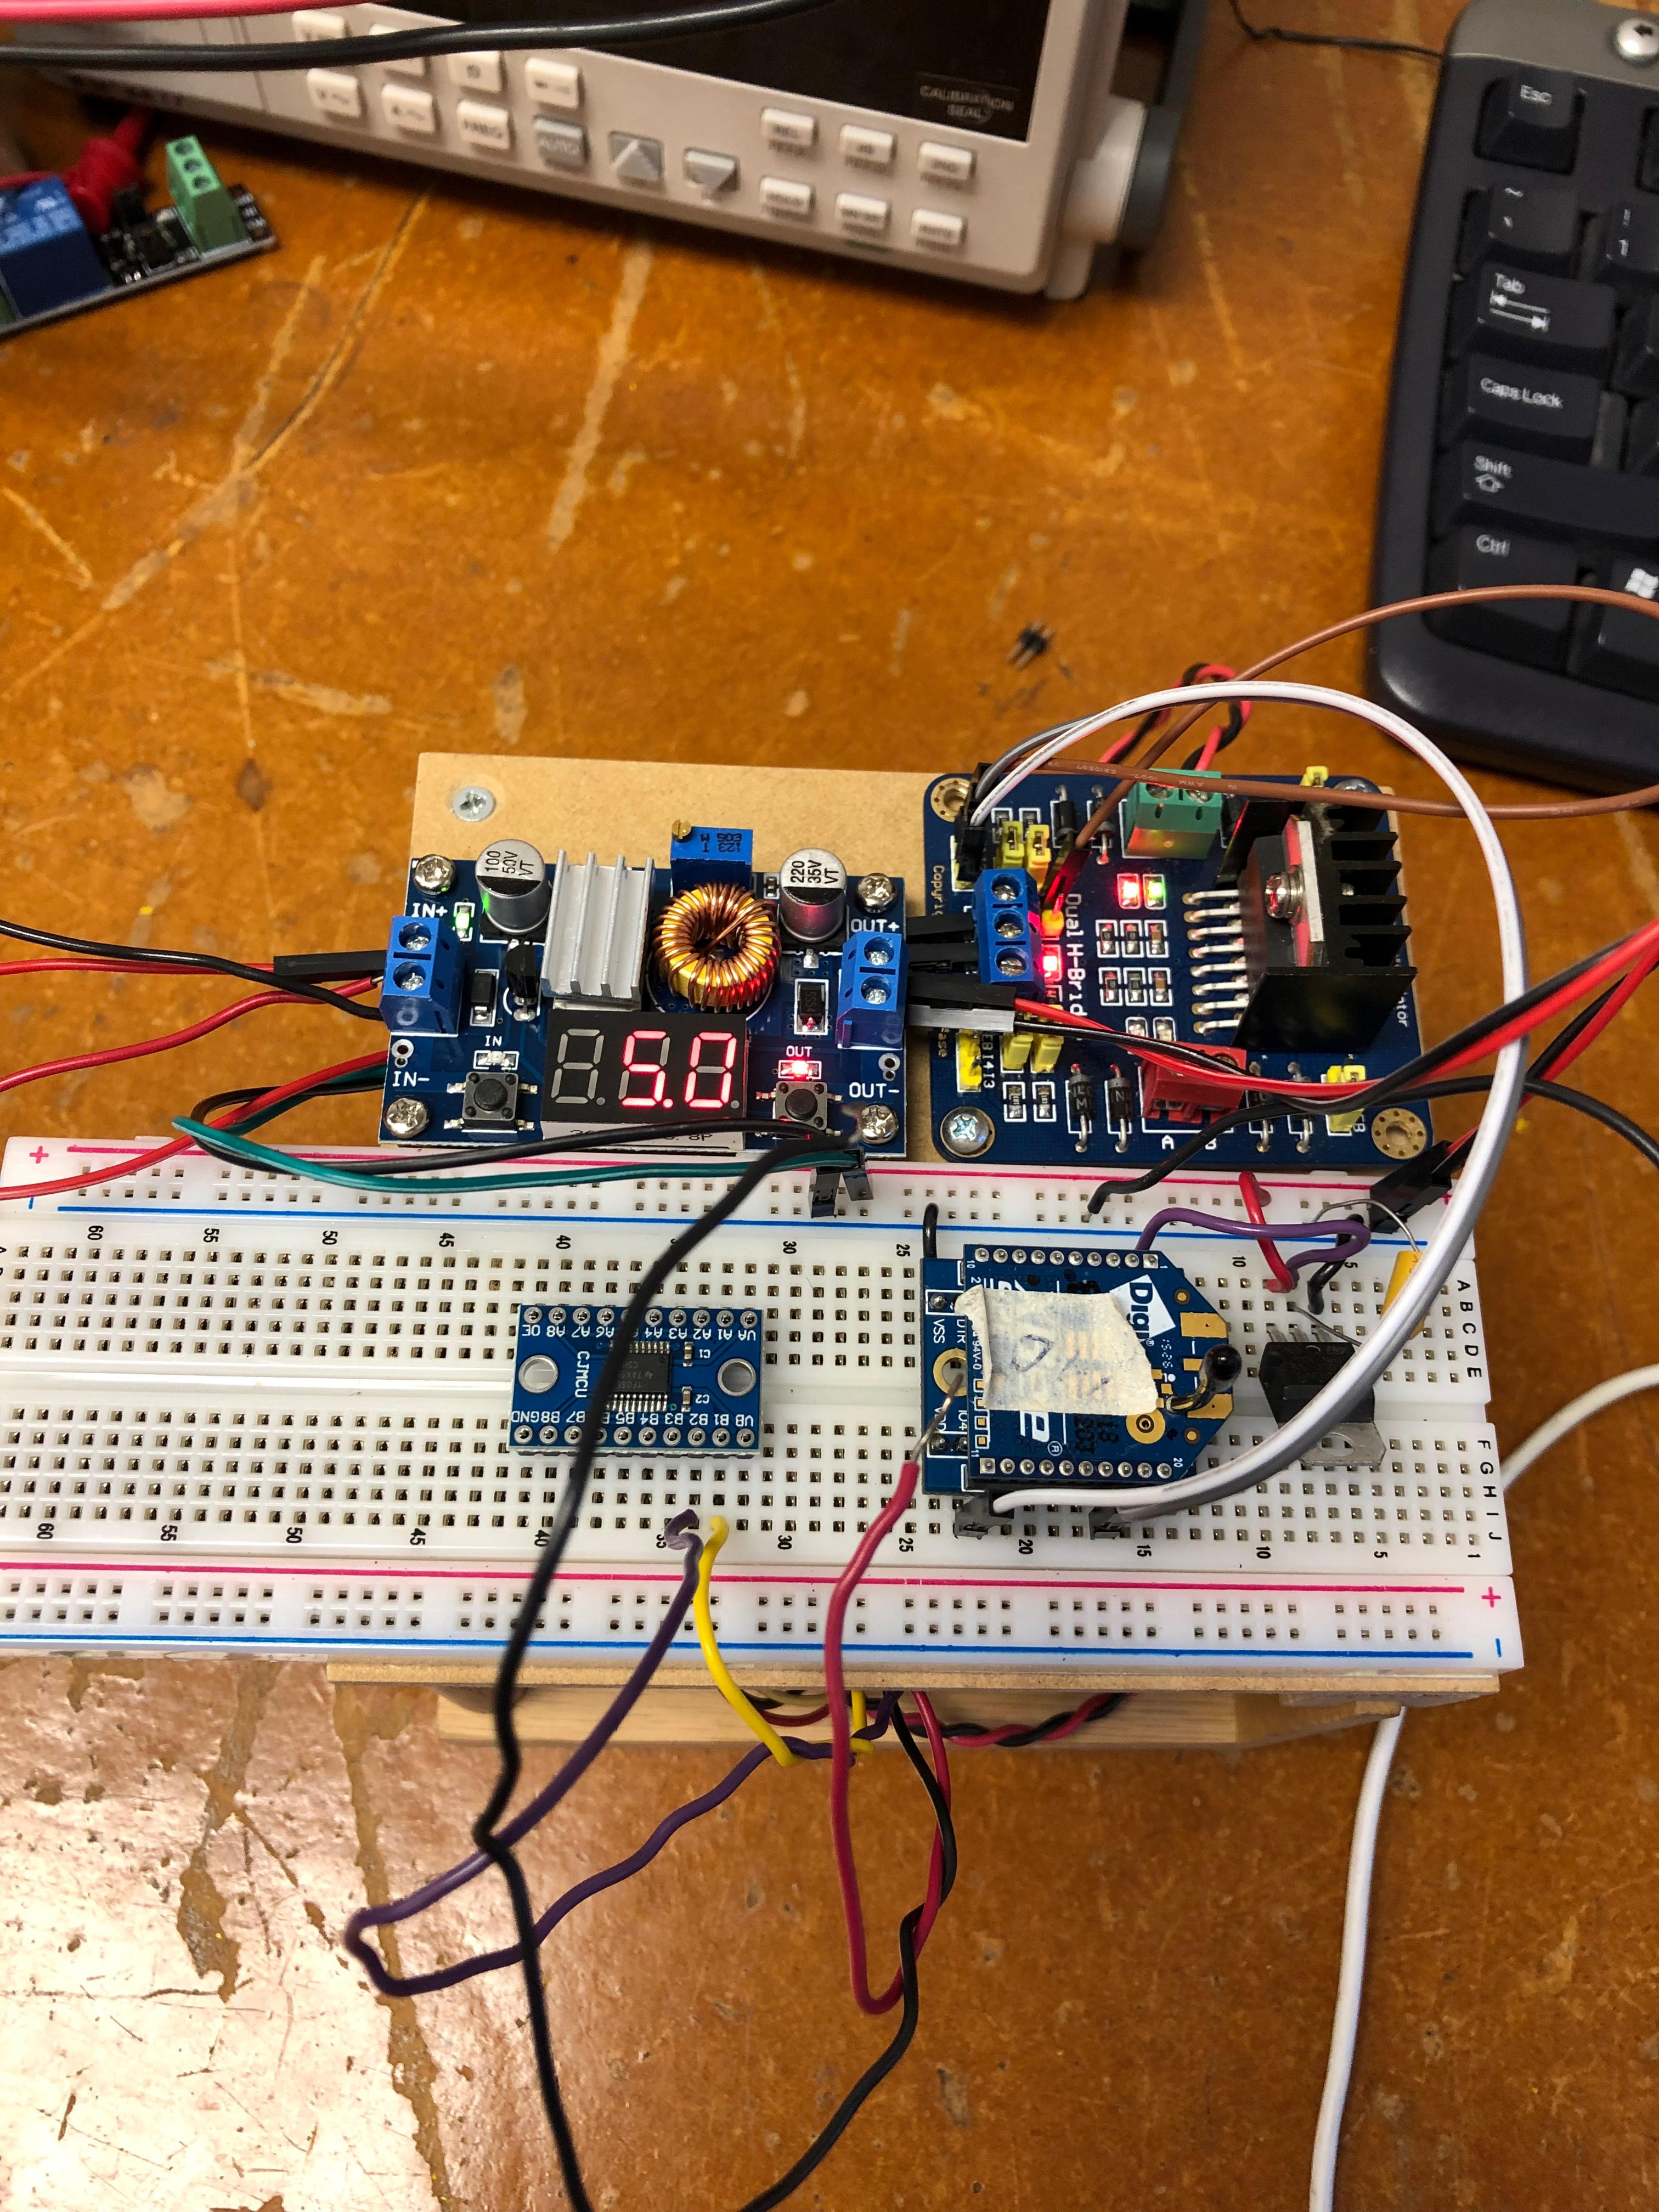
\includegraphics[scale=.04]{figs/img/Circuit1027.jpg}
     \caption{Remote Circuit 10/27/18}
     \label{fig:RemoteCircuit10/27}
    \end{figure}
\end{frame}



 \begin{frame}{Engineering Efforts}{Experimental Activities}
\begin{itemize}

\item XBee S2C radio module

     \begin{itemize}

         \item Receive motor direction commands

         \item Toggle H-Bridge pins

         \item Relay encoder positional data to central node

     \end{itemize}

\item L298 H-bridge
     \begin{itemize}
            \item Supply motor power
            \item control motor rotation direction
     \end{itemize}

\item Pittman 24v DC motor
     \begin{itemize}
         \item Close/ open curtains
     \end{itemize}

\item Optical encoder
     \begin{itemize}
         \item Measure and relay positional data
     \end{itemize}
\item Buck/Boost Converter
    \begin{itemize}
        \item Allow for a single power source to remote node
        \item Bucks incoming 20V line down to 5V for motor driver, XBee module, and encoder logic  
    \end{itemize}

\end{itemize}

\end{frame} 
  
\begin{frame}{Engineering Efforts}{Experimental Activities}
  \begin{figure}
    \centering
    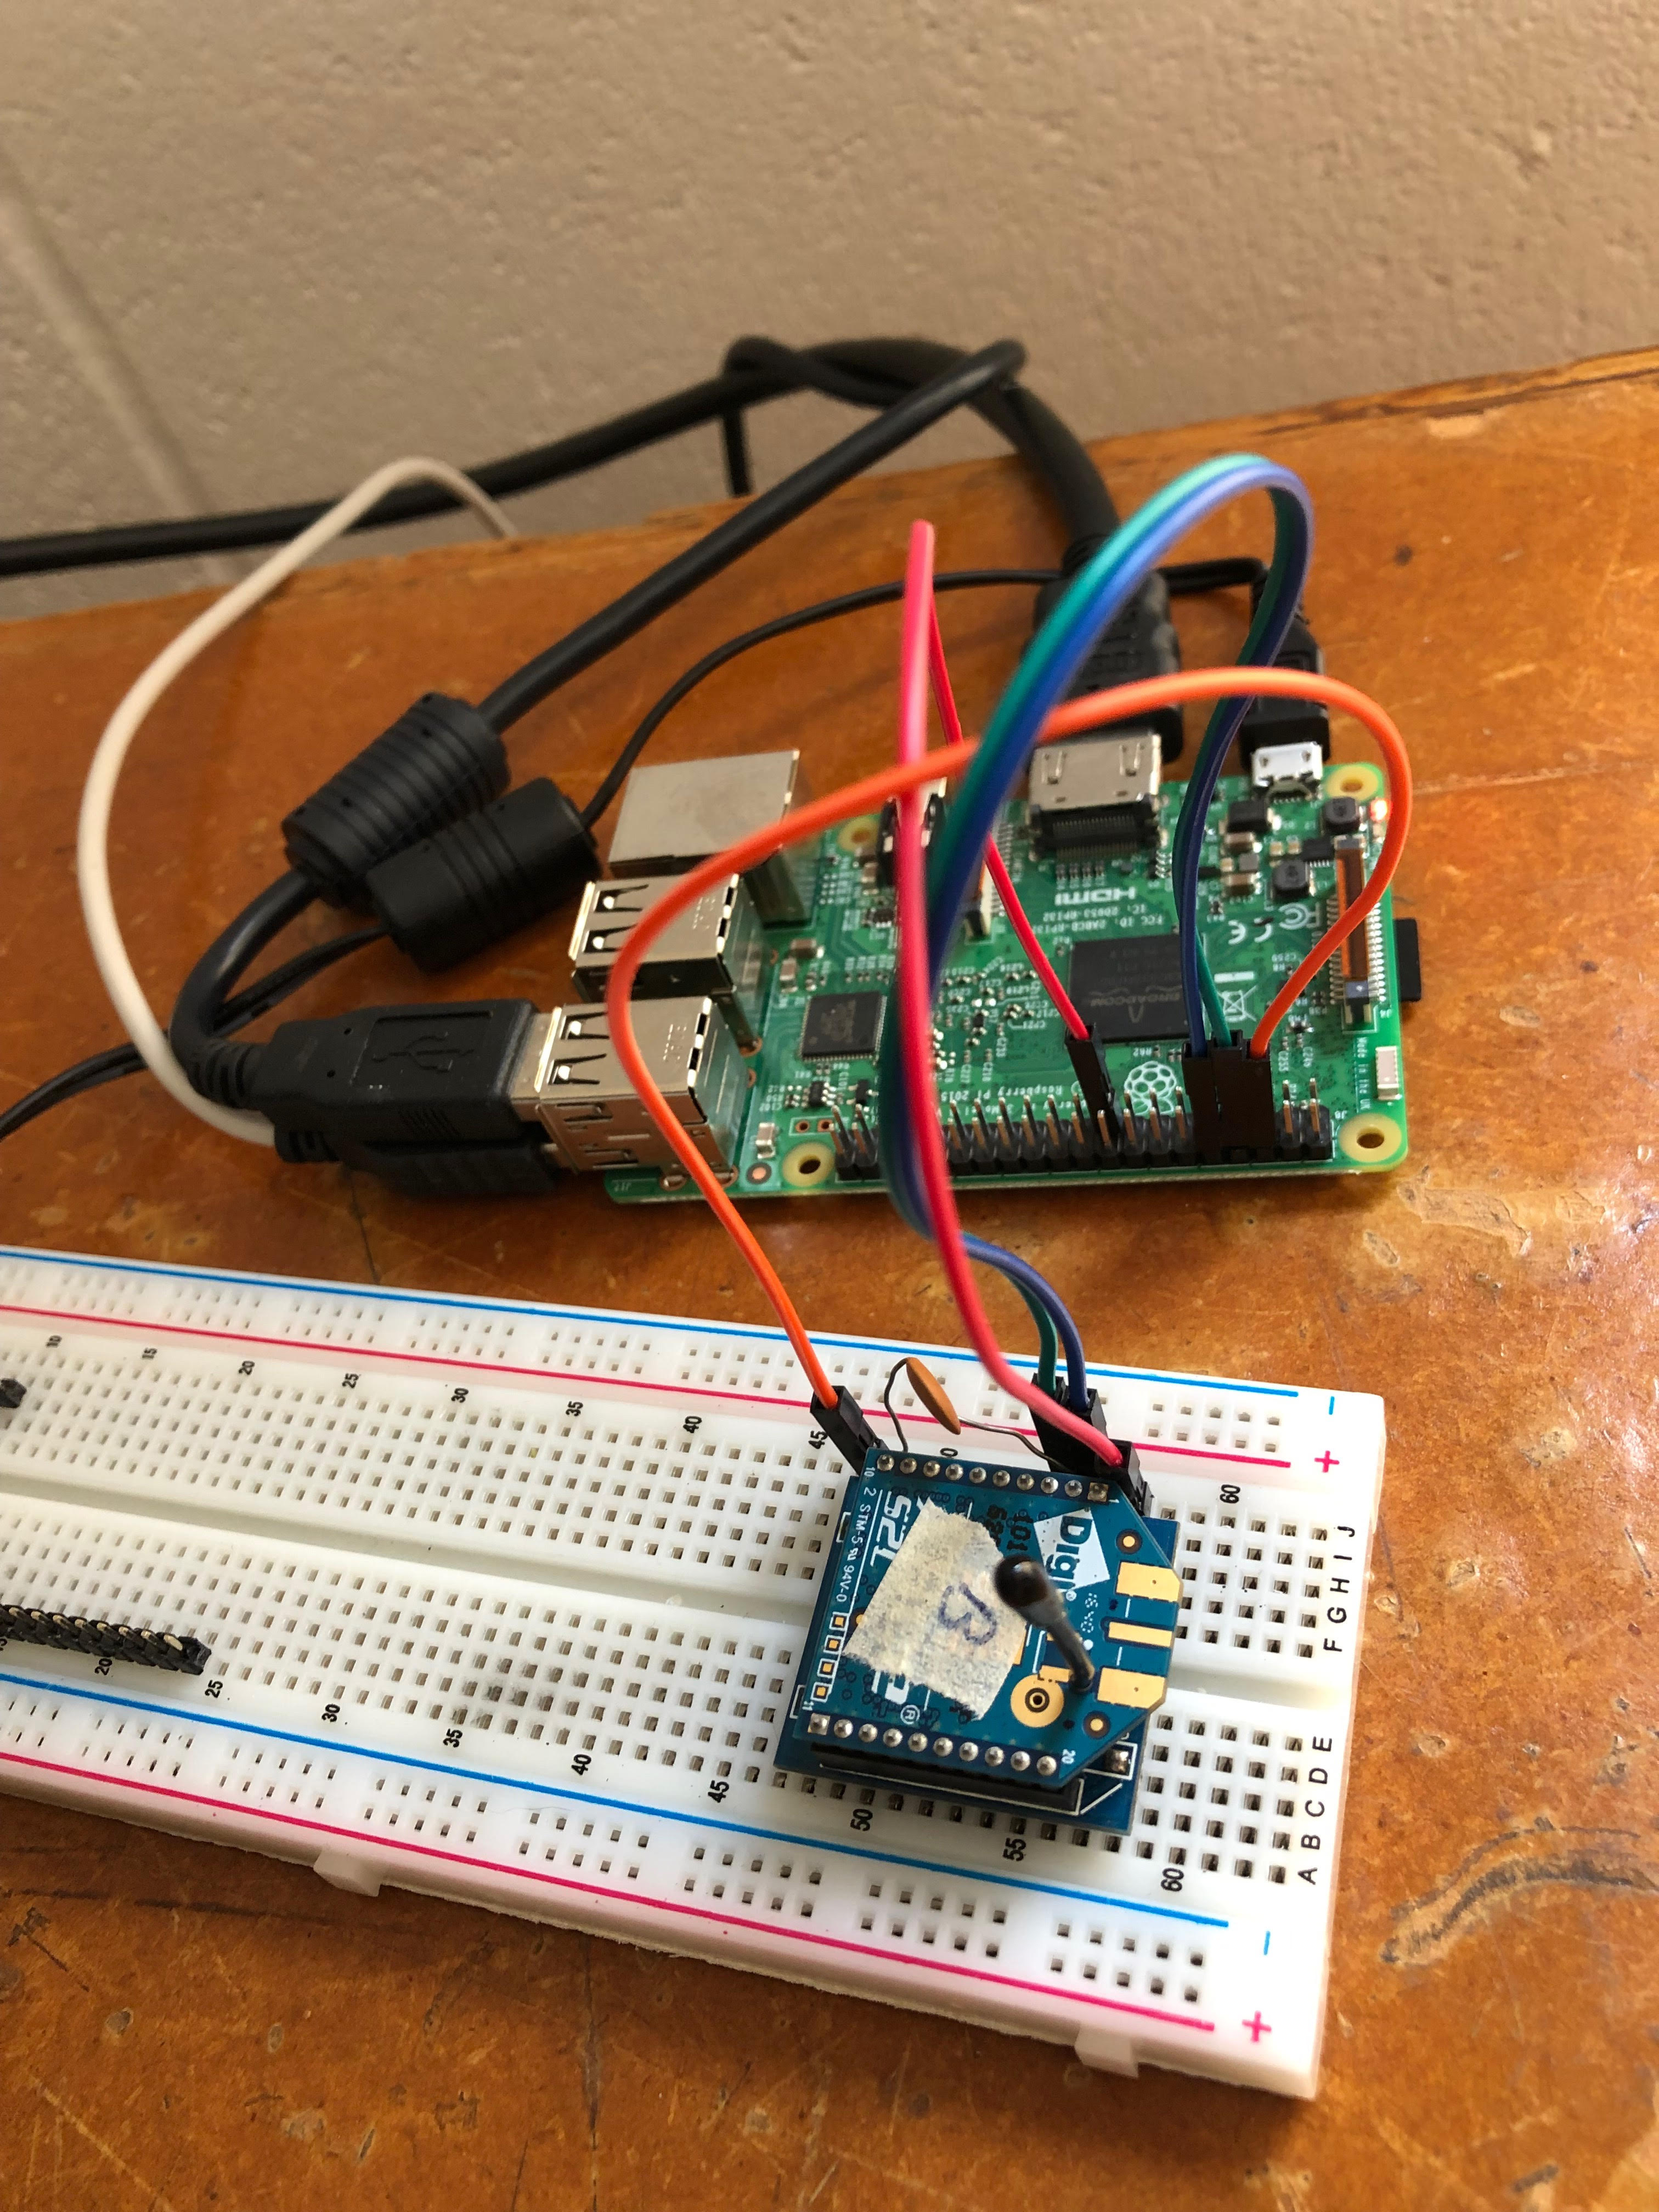
\includegraphics[scale=.04]{figs/img/PiXBee.jpg}
    \caption{Raspberry Pi Central Node}
    \label{fig:RpiCentralNode}
\end{figure}
\end{frame}

\begin{frame}{Engineering Efforts}{Experimental Activities}

 
\begin{itemize}
        \item Raspberry Pi Model 3B
        \begin{itemize}
            \item Connect to BEMOSS
            \item TX pin to transmit commands
            \item RX pin to recieve encoder data 

        \end{itemize}  
        \item Python Script:
            \begin{itemize}
            \item Transmit remote AT commands to XBee Module
            \item Process encoder data and send stop start command
            \end{itemize}

        \item XBee S2C radio module 
            \begin{itemize} 
                \item Coordinator XBee
        \end{itemize}
    \end{itemize}

\end{frame} 

\begin{frame}{Engineering Efforts}{Design}
  BEMOSS video presentation 
\end{frame}


\begin{frame}{Engineering Efforts}{Experimental Activities}


    \begin{itemize}
        \item Future work includes:
            \begin{itemize}
                \item Utilize logic converters to allow data exchange between the 5V logic H-bridge and encoder to the 3.3v logic XBee module (Pictured in "Remote Circuit 10/27/18)
                \item Employ I2C protocol in place of XBee radio communication between nodes (cheaper communication method)
                \item Implement feedback control using the motor encoder to control the position and speed of the motor
                \item Further energy efficiency by only powering the encoder during times of motor rotation (through use of relays)
 
    \end{itemize}
    \end{itemize}

\end{frame} 






%----------------------------------

\section{Parts List}

\begin{frame}{Parts List}{}
  \begin{table}
\centering
\begin{tabular}{|c|c|c|}
    \hline
    Part & Price & Quantity \\
    \hline 
    XBee Interface Board & \$5.31 & 1 \\
    \hline
    8 Channel Logic Converter & \$5.99 & 1 \\
    \hline
    $3.3~[\volt]$ Relay Board & \$11.90 & 1\\
    \hline 
    Buck/ Boost Converter & \$9.99 & 1\\
    \hline 
    WeMo Smart Plug & \$ 27.90 & 2\\
    \hline
\end{tabular}
\caption{List of ordered parts}
\label{tab:ordparts}
\end{table}
\end{frame}

%----------------------------------

\section{ECE 499 Deliverables}

\subsection{Division of Labor}
%BOB will do schedule for completion
\begin{frame}{Deliverables}{Division of Labor}
  \begin{itemize}
      \item Jordan 
      \begin{itemize}
          \item Develop accurate models using Simscape
          \item Algorithm for BEMOSS
          \item Machine learning research and implementation
      \end{itemize}
      \item Reece
      \begin{itemize}
          \item Interfacing a new device
          \item Motor driver configuration
      \end{itemize}
      \item Robert
      \begin{itemize}
          \item BEMOSS 
          \item Implement Reece and Jordan's work
      \end{itemize}
  \end{itemize}


\end{frame}

%----------------------------------

\subsection{Schedule for Completion}

\begin{frame}{Deliverables}{Schedule for Completion}
  Fall Semester 2018
  \begin{itemize}
        \item Working BEMOSS - September 2018
        \item Transmit AT command via XCTU - October 2018
        \item Transmit AT command via python - November 2018
        \item Adaptive HVAC Control Algorithm - December 2018
        \end{itemize}
\end{frame}

\begin{frame}{Deliverables}{Schedule for Completion}
    Spring Semester 2019
    \begin{itemize}

        \item Interface new device - March 2019
        \item Implement Machine learning - April 2019
        \item Have device supported by BEMOSS - April 2019
    \end{itemize}
\end{frame}


%----------------------------------

\section*{Summary}

\begin{frame}{Summary}
  \begin{itemize}
  \item
    Introduce a new supported device within BEMOSS
  \item
    Configure BEMOSS to work on a single board computer like raspberry pi
  \item 
  Develop an algorithm for BEMOSS to determine energy consumption and energy saved
  \end{itemize}
\end{frame}
\section{Discussion}

\begin{frame}{Discussion}{}
  Questions?
\end{frame}

%----------------------------------



% You can reveal the parts of a slide one at a time
% with the \pause command:
%\begin{frame}{Second Slide Title}
%  \begin{itemize}
%  \item {
%    First item.
%    \pause % The slide will pause after showing the first item
%  }
  %\item {   
  %  Second item.
 % }
  % You can also specify when the content should appear
  % by using <n->:
 % \item<3-> {
 %   Third item.
 % }
%  \item<4-> {
%    Fourth item.
 % }
  % or you can use the \uncover command to reveal general
  % content (not just \items):
%  \item<5-> {
%    Fifth item. \uncover<6->{Extra text in the fifth item.}
%  }
%  \end{itemize}
%\end{frame}

%\section{Second Main Section}

%\subsection{Another Subsection}

%\begin{frame}{Blocks}
%\begin{block}{Block Title}
%You can also highlight sections of your %presentation in a block, with it's own %title
%\end{block}
%\begin{theorem}
%There are separate environments for %theorems, examples, definitions and proofs.
%\end{theorem}
%\begin{example}
%Here is an example of an example block.
%\end{example}
%\end{frame}

% Placing a * after \section means it will not show in the
% outline or table of contents.




% All of the following is optional and typically not needed. 
\appendix
\section<presentation>*{\appendixname}
\subsection<presentation>*{For Further Reading}
% \bibliographystyle{plain}
% \bibliography{}
\begin{frame}[allowframebreaks]
  \frametitle<presentation>{For Further Reading}
    
  \begin{thebibliography}{10}
    
  \beamertemplatebookbibitems
  % Start with overview books.


 
    
  \beamertemplatearticlebibitems
  % Followed by interesting articles. Keep the list short. 
  \bibitem{Ferreira2012}
    P. M. Ferreira
    \newblock{Neural networks based predictive control for thermal comfort and energy savings in public buildings}/
    \newblock{} Energy and Buildings, 2012
  \bibitem{Reppa 2015}
    V. Reppa
    \newblock {\em A Distributed Architecture for HVAC Sensor Fault Detection and Isolation}.
    \newblock IEEE Transactions on Control Systems Technology, 2015.
  \bibitem{Zhang2016}
    X. Zhang
    \newblock{\em Deploying IoT devices to make buildings smart: Performance evaluation and deployment experience}.
    \newblock 2016 IEEE 3rd World Forum on Internet of Things (WF-IoT)
    
  \end{thebibliography}
\end{frame}

\end{document}



%%% Local Variables:
%%% mode: latex
%%% TeX-master: t
%%% End:
